%#################### 4.1 ####################
	\begin{table}[h!]
	\begin{tabular}{c | c}
	\begin{minipage}[m]{0.4\textwidth}
	\enum{
	\begin{tcolorbox}[colback=white!100,colframe=red!75!black,width=7cm,righttitle=0.5cm,subtitle style={boxrule=0.4pt, colback=yellow!50!red!25!white},title= \bf{1}\hfill  \bf{22}]
		\begin{center}\bf{333}\end{center}
		\tcblower
		\href{https://tools.ietf.org/doc/texlive-doc/latex/tcolorbox/tcolorbox.pdf}{Source}
		\end{tcolorbox}}{4.1}
	\end{minipage}
	&
	\begin{minipage}[m]{0.55\textwidth}
	\begin{lstlisting}[basicstyle=\scriptsize]
	\PassOptionsToPackage{svgnames}{xcolor}
	\documentclass[twocolumn,a4paper]{article}
	\usepackage{tcolorbox}
	\tcbuselibrary{skins,breakable}
	\usetikzlibrary{shadings,shadows}%preambule
	\begin{tcolorbox}[colback=white!100,colframe=red!75!black,width=7cm,righttitle=0.5cm, subtitle style={boxrule=0.4pt,colback=yellow!50!red!25!white},title= \bf{1}\hfill \bf{22}]
		\begin{center}\bf{333}\end{center}
		\tcblower
		\href{https://tools.ietf.org/doc/texlive-doc/latex/tcolorbox/tcolorbox.pdf}{URL}
	\end{tcolorbox}
	\end{lstlisting}
	\end{minipage}
	\end{tabular}
	\end{table}

%#################### 4.2 ####################
	\begin{table}[h!]
	\begin{tabular}{c | c}
	\begin{minipage}[m]{0.4\textwidth}
	\enum{The \mybox[green]{quick} brown \mybox{fox} \mybox[blue]{jumps} over the
	\mybox[green]{lazy} \mybox{dog}.\par
	The \xmybox[green]{quick} brown \xmybox{fox} \xmybox[blue]{jumps} over the
	\xmybox[green]{lazy} \xmybox{dog}.}{4.2}
	
	\end{minipage}
	&
	\begin{minipage}[m]{0.55\textwidth}
	\begin{lstlisting}[basicstyle=\footnotesize]
	\usepackage{tcolorbox}
	\newtcbox{\mybox}[1][red]{on line,
	arc=0pt,outer arc=0pt,colback=#1!10!white,colframe=#1!50!black,
	boxsep=0pt,left=1pt,right=1pt,top=2pt,bottom=2pt,
	boxrule=0pt,bottomrule=1pt,toprule=1pt}
	\newtcbox{\xmybox}[1][red]{on line,
	arc=7pt,colback=#1!10!white,colframe=#1!50!black,
	before upper={\rule[-3pt]{0pt}{10pt}},boxrule=1pt,
	boxsep=0pt,left=6pt,right=6pt,top=2pt,bottom=2pt}
	%usage---> \xmybox[YOUR_colour]{YOUR_text}
			  %\mybox[YOUR_colour]{YOUR_text}
	\end{lstlisting}
	\end{minipage}
	\end{tabular}
	\end{table}

%#################### 4.3 ####################
	\begin{table}[h!]
	\begin{tabular}{c | c}
	\begin{minipage}[m]{0.4\textwidth}
	\enum{
	Here You can see \mylib{\href{https://texdoc.org/serve/tcolorbox.pdf/0}{more examples}} and learn something new.}{4.3}
	\end{minipage}
	&
	\begin{minipage}[m]{0.55\textwidth}
	\begin{lstlisting}[basicstyle=\footnotesize]
	\usepackage[many]{tcolorbox}
	\newtcbox{\mylib}{enhanced,nobeforeafter,tcbox raise base,boxrule=0.4pt,top=0mm,bottom=0mm,
	  right=0mm,left=4mm,arc=1pt,boxsep=2pt,before upper={\vphantom{dlg}},
	  colframe=green!50!black,coltext=green!25!black,colback=green!10!white,
	  overlay={\begin{tcbclipinterior}\fill[green!75!blue!50!white] (frame.south west)
	    rectangle node[text=white,font=\sffamily\bfseries\tiny,rotate=90] {TYP} ([xshift=4mm]frame.north west);\end{tcbclipinterior}}}
	\begin{document}

	\mylib{recieve}
	\end{lstlisting}
	\end{minipage}
	\end{tabular}
	\end{table}

%#################### 4.4 ####################
	\begin{table}[h!]
	\begin{tabular}{c | c}
	\begin{minipage}[m]{0.4\textwidth}
	\enum{
	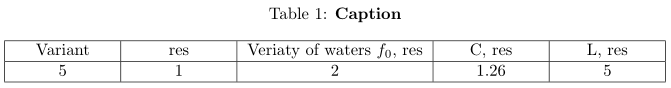
\includegraphics[width=1\linewidth]{4.5.png}
	\textit{\small{table with the desired length, a command was also created to create a new cell view in the table.}}}{4.4}
	\end{minipage}
	&
	\begin{minipage}[m]{0.55\textwidth}
	\begin{lstlisting}[basicstyle=\footnotesize]
	\usepackage{graphicx}
	\usepackage{tabularx}
	\newcolumntype{Y}{>{\centering\arraybackslash}X}
	\begin{document}
	\begin{table}[h!]
	\begin{center}
	\caption{\textbf{Caption}}
	  \begin{tabularx}{14cm}{|Y|Y|c|Y|Y|}
	  \hline
	  Variant & res & Veriaty of waters $f_0$, res & C, res & L, res\\
	  \hline
	  5       &     1   &               2               & 1.26 & 5\\
	  \hline
	  \end{tabularx}
	\end{center}
	\end{table}
	\end{lstlisting}
	\end{minipage}
	\end{tabular}
	\end{table}

%#################### 4.5 ####################
\begin{table}[h!]
	\begin{tabular}{c | c}
	\begin{minipage}[m]{0.4\textwidth}
	\enum{
	\circled[fill=amber,draw=black]{1} 
	\circled[fill=babyblue,draw=black]{2} 
	\circled[fill=green,draw=black]{3}  
	$\cdots$\circled[fill=green!75!blue!50!white,draw=black]{4} 
	\circled[fill=orange,draw=black]{5} 
	\circled[fill=purple!70!white,draw=black]{6}}{4.5}
	\end{minipage}
	&
	\begin{minipage}[m]{0.55\textwidth}
	\begin{lstlisting}[basicstyle=\footnotesize]{tex}
	\usepackage{tikz}
	\usepackage[framemethod=TikZ]{mdframed}
	\usepackage{xcolor}
	\usetikzlibrary{calc}
	\makeatletter
	\newlength{\mylength}
	\xdef\CircleFactor{1.1}
	\setlength\mylength{\dimexpr\f@size pt}
	\newsavebox{\mybox}
	\newcommand*\circled[2][draw=blue]{\savebox\mybox{\vbox{\vphantom{WL1/}#1}}\setlength\mylength{\dimexpr\CircleFactor\dimexpr\ht\mybox+\dp\mybox\relax\relax}\tikzset{mystyle/.style={circle,#1,minimum height={\mylength}}}	\tikz[baseline=(char.base)]
	\node[mystyle] (char) {#2};}
	\makeatother
	\definecolor{amber}{rgb}{1.0, 0.75, 0.0}
	\definecolor{babyblue}{rgb}{0.54, 0.81, 0.94}
	usage -->  \circled[fill=amber,draw=black]{1} 
	\end{lstlisting}
	\end{minipage}
	\end{tabular}
	\end{table}

%#################### 4.6 ####################
	\begin{tabular}{c | c}
	\begin{minipage}[m]{0.4\textwidth}
	\enum{
	\begin{caja}[title=warning]
	Here is some text 
	\end{caja}}{4.6}
	\end{minipage}
	&
	\begin{minipage}[m]{0.55\textwidth}
	\begin{lstlisting}[basicstyle=\footnotesize]{tex}
\usepackage[utf8]{inputenc}
\usepackage[T1]{fontenc}
\usepackage[most]{tcolorbox}
\definecolor{orang}{RGB}{255,155,0}
\newtcolorbox[auto counter,number within=section]{caja}[1][]{
enhanced jigsaw,colback=white,colframe=orang,coltitle=orang,
fonttitle=\bfseries\sffamily,
sharp corners,
detach title,
leftrule=10mm,
% What you need %%%%%%%%%%%%
underlay unbroken and first={\node[below,text=black,anchor=east]
at ([xshift=-5.5pt]interior.base west) {\Huge  \textbf{!}};},
%%%%%%%%%%%%%%%%%%%%%%%%
breakable,pad at break=1mm,
#1,
code={\ifdefempty{\tcbtitletext}{}{\tcbset{before upper={\tcbtitle\par\medskip}}}},}
\begin{document}
\begin{caja}[title=warning]
The vertical alignment settings 
\end{caja}
\end{document}	
	\end{lstlisting}
	\end{minipage}
	\end{tabular}

\vspace{0.2cm}	

%#################### 4.7 ####################
	\begin{tabular}{c | c}
	\begin{minipage}[m]{0.4\textwidth}
	\enum{
	\begin{tcolorbox}[enhanced,sharp corners,
  width={5cm},
  colback=white,
  overlay={\node at (frame.south east) {\includegraphics[scale=0.1]{example-image-a}};} ]
Sample text here.
\end{tcolorbox}}{4.7}
	\end{minipage}
	&
	\begin{minipage}[m]{0.55\textwidth}
	\begin{lstlisting}[basicstyle=\footnotesize]{tex}
\documentclass{article}
\usepackage[most]{tcolorbox}
\usepackage{graphicx}
\begin{document}
\begin{tcolorbox}[enhanced,sharp corners,
  width={5cm},
  colback=white,
  overlay={\node at (frame.south east) {\includegraphics[scale=0.1]{example-image-a}};} ]
Sample text here.
\end{tcolorbox}
\end{document}	
	\end{lstlisting}
	\end{minipage}
	\end{tabular}

%#################### 4.8 ####################
	\begin{tabular}{c | c}
	\begin{minipage}[m]{0.4\textwidth}
	\enum{
    
     
    \makegapedcells
        \begin{tabular}{|c|c|c| }
        \hline
    all&in&cells\\ \hline
    are&centered&vertically\\ \hline
    and&horisontally&\\ \hline
     
    \end{tabular}
     
	 }{4.8}
	\end{minipage}
	&
	\begin{minipage}[m]{0.55\textwidth}
	\begin{lstlisting}[basicstyle=\footnotesize]{tex}
   \documentclass{article}
    \usepackage{float}
    \usepackage{array, makecell}
    \setcellgapes{5pt}

    \begin{document}
    \begin{table}[H]
    \center
    \makegapedcells
        \begin{tabular}{|c|c|c|c|}
        \hline
    1&1&1&1\\ \hline
    1&1&1&1\\ \hline
    1&1&1&1\\ \hline
     
    \end{tabular}
    \end{table}

    \end{document}
	\end{lstlisting}
	\end{minipage}
	\end{tabular}






